\section{Goals and Contribution}

The core of the problem is that the Sampling Broker is a centralized entity. In general, the problem of a centralized system is solved by replacing it with a distributed system. Hence, in this case, the idea is to replace the centralized broker with a distributed broker. To the best of our knowledge currently there exist no implementation of SSPS on any of the available distributed brokers. 

There are several open-source distributed brokers like Apache ActiveMQ Artemis, Apache Kafka and so on. The first part of this thesis would be to study the different open-source distributed brokers and select one among them for implementing the SSPS. Secondly, once an appropriate broker has been chosen, the architecture of the broker needs to be understood in order to extend it to incorporate the SSPS. Then, we design and implement a prototypical extension for the SSPS. Figure \ref{figures:dist_ssps} depicts the design of the Sampling Broker in the case of a distributed broker. In comparison to Figure \ref{figures:ssps} it can be seen that now there are several instances of the sampling broker instead of only one instance.

\makeatletter
\setlength{\@fptop}{0pt}
\makeatother

\begin{figure}[t!]
\centering
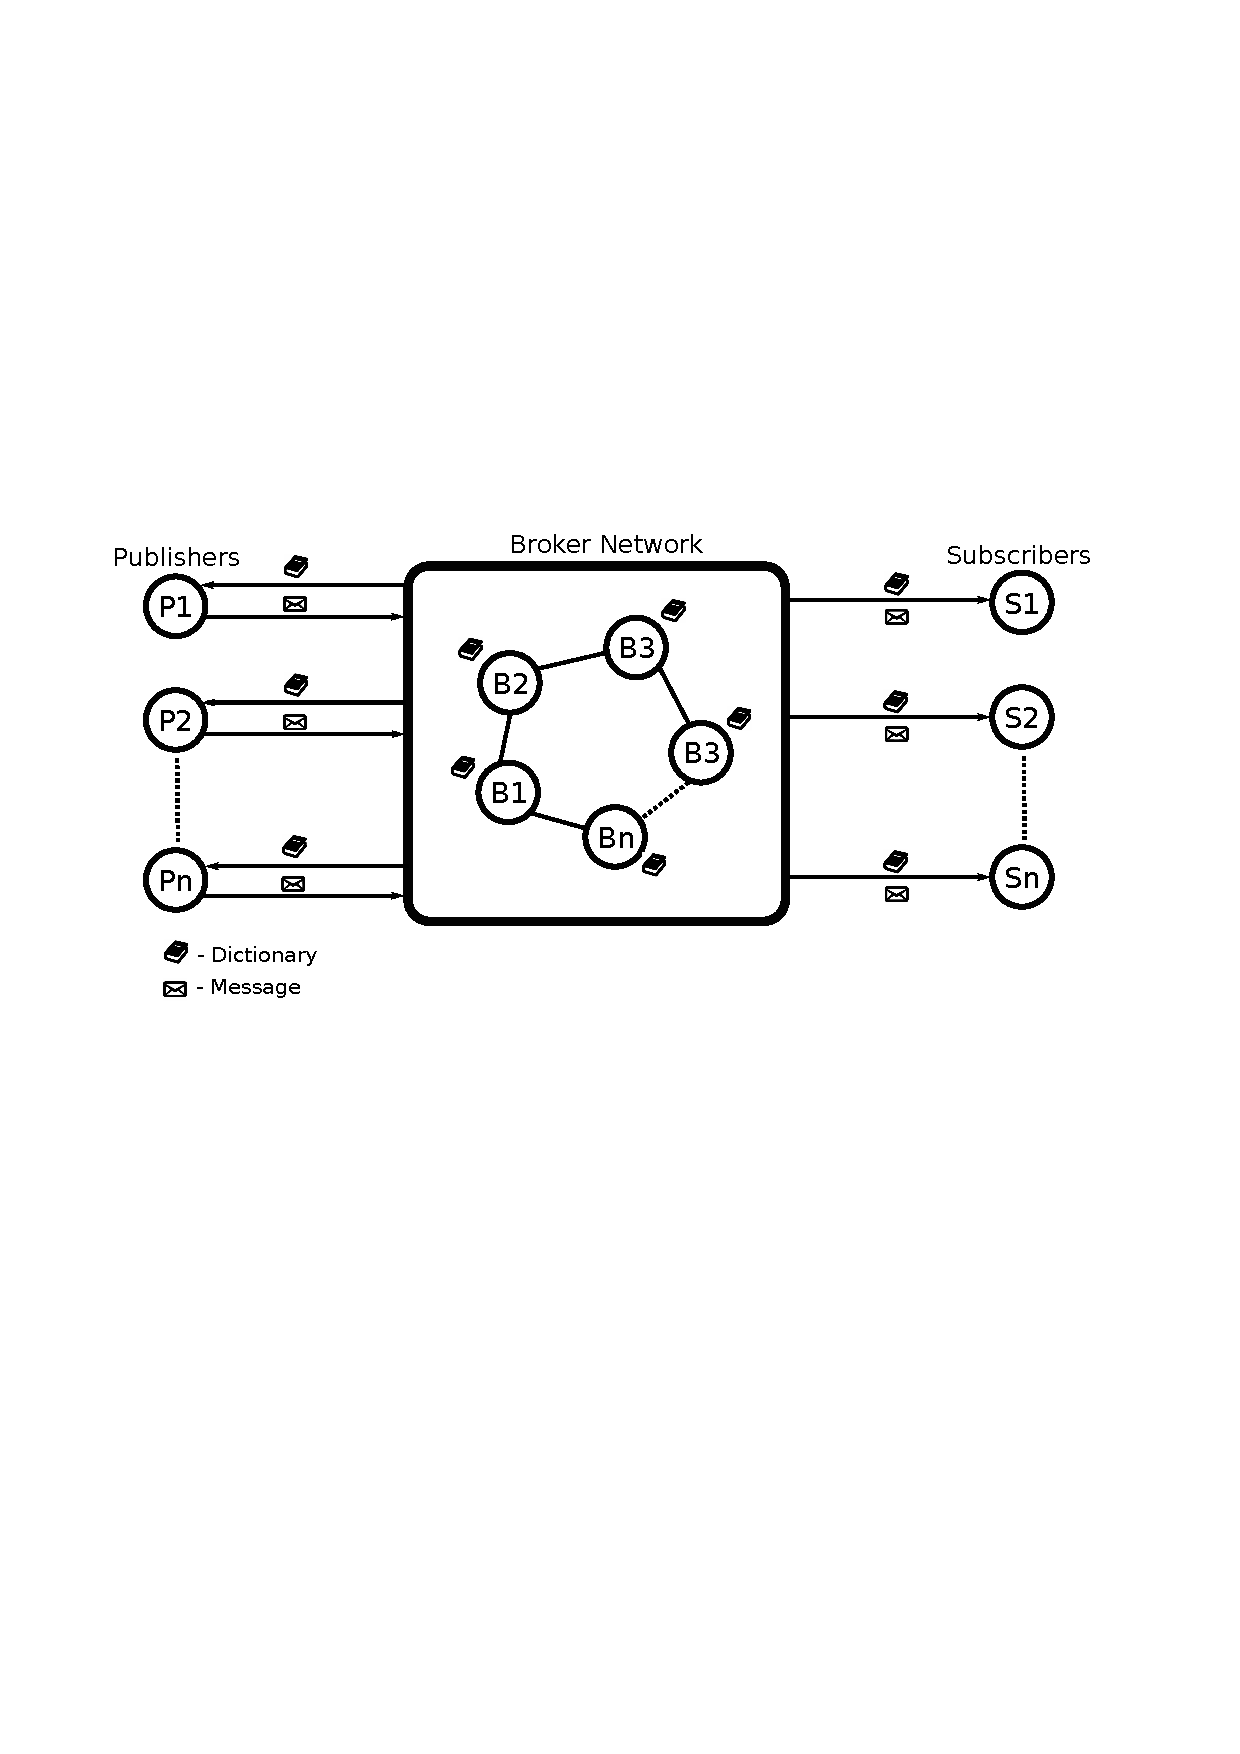
\includegraphics[keepaspectratio, width=.7\textwidth]{dist_ssps.pdf}
\caption{SSPS in a distributed broker}\label{figures:dist_ssps}
\end{figure}

Once the implementation is complete, we test our prototypical implementation to get performance aspects such as throughput, CPU and memory usage and behavioral aspects such as the effect of SSPS in the case of failover. Finally, we create an android application to demonstrate the working of SSPS. In brief, the Android application would provide the provision to subscribe to a set of topics. Each topic would correspond to messages being received by the Android application in different formats such as JSON, XML, and CSV. The messages would contain location coordinates which will be displayed on a map. The Android application would also demonstrate the throughput comparison with and without the use of SSPS.
